\documentclass[UTF8]{ctexart}
\usepackage{mathtools,booktabs}
\usepackage{graphicx}
%添加路径,图片的搜索路径
\graphicspath{{figures/}}
\usepackage{listings} 
\usepackage{xcolor}
\lstset{
	language=c,  %代码语言使用的是matlab
	frame=shadowbox, %把代码用带有阴影的框圈起来
	rulesepcolor=\color{red!20!green!20!blue!20},%代码块边框为淡青色
	keywordstyle=\color{blue!90}\bfseries, %代码关键字的颜色为蓝色,粗体
	commentstyle=\color{red!10!green!70}\textit,    % 设置代码注释的颜色
	showstringspaces=false,%不显示代码字符串中间的空格标记
	numbers=left, % 显示行号
	numberstyle=\tiny,    % 行号字体
	stringstyle=\ttfamily, % 代码字符串的特殊格式
	breaklines=true, %对过长的代码自动换行
	extendedchars=false,  %解决代码跨页时,章节标题,页眉等汉字不显示的问题
	%   escapebegin=\begin{CJK*},escapeend=\end{CJK*},      % 代码中出现中文必须加上,否则报错
	texcl=true}


\begin{document}
	
	\title{八股文背诵合集}
	\author{The Sea and Sheng}
	\maketitle
	
	\tableofcontents
	\newpage
	
	\section{Spring}
	%\subsection{二级标题}
	\subsubsection{Spring 框架能带来哪些好处}

	\begin{enumerate}
		\item Dependency Injection(DI) 依赖注入 是的构造器和JavaBean properties文件中的依赖关系一目了然.
		\item IoC容器更加趋向于轻量级.
	\end{enumerate}
	
	\subsubsection{什么是控制反转(IOC)}
	\begin{enumerate}
		\item 
		控制反转简单来说, 以前程序开发的时候, 是由程序员通过new来生成对象. 在使用控制反转的情况下, 对象的实例化由Spring框架中的IoC容器来控制对象的创建; 
		\item 由容器来管理这些对象的生命周期.
		\item Spring中的org.springframework.beans包和org.springframework.conext包构成了Spring框架Ioc的基础. 主要使用文件 applicationContext.xml 来进行配置.
	\end{enumerate}

	\subsubsection{什么是依赖注入?}
	\begin{enumerate}
		\item Spring 通过反射来实现依赖注入
		\item 当我们需要某个功能比如Connection, 至于Connection怎么构造, 何时构造我们不需要知道. 在系统运行时, Spring会在适当的时候制造一个Connection, 我们需要一个Connection, 这个Connection是由Sping注入到A中. 
	\end{enumerate}
\subsubsection{Spring 对对象进行创建流程}
class对象反射 ---> 实例化 ---> 生成对象 ---> 属性填充(依赖注入)  ---> 初始化(afterPropertiesSet) ---> AOP ---> 代理对象(cglib) ---> bean
\subsubsection{简单阐述SpringMVC的流程}
	SpringMVC是一个基于Java的实现了MVC设计模式的请求驱动类型的轻量级Web框架, 通过把Model, View, Controller分离, 将web层进行职责解耦, 把复杂的web应用分成逻辑清晰的几部分, 简化开发.
\par
(1) 用户发送请求到前端控制器DispatcherServlet;
\par
(2) DispatcherServlet 收到请求后, 调用HandlerMapping处理器映射器, 请求获取Handle
\par
(3) 处理器映射器更具请求url找到具体的处理器, 生成处理器对象以及处理器拦截器(如果有则生成)一并返回给DispatcherServlet;
\par
(4) DispatcherServlet 调用HandlerAdapter处理器适配器;
\par
(5) HandlerAdapter 经过适配调用具体处理器(Handler, 也叫后端控制器);
\par
(6) Handler 执行完成返回ModelAndView;
\par
(7) HandlerAdapter将Handler执行结果ModelAndView返回给DispatcherServlet;
\par
(8) DispatcherServlet将ModelAndView传给ViewResolver视图解析器进行解析;
\par
(9) ViewResolver解析后返回具体View
\par
(10) DispatcherServlet对View进行渲染视图(即将模型数据填充到视图中)
\par
(11) DispatcherServlet响应用户.
\par
简单来说, 我们需要开发的就是 == 开发处理器(Handler,即我们的Controller, 对于视图jsp我们前后端分离之后也不用写了.
\begin{figure}
	\centering
	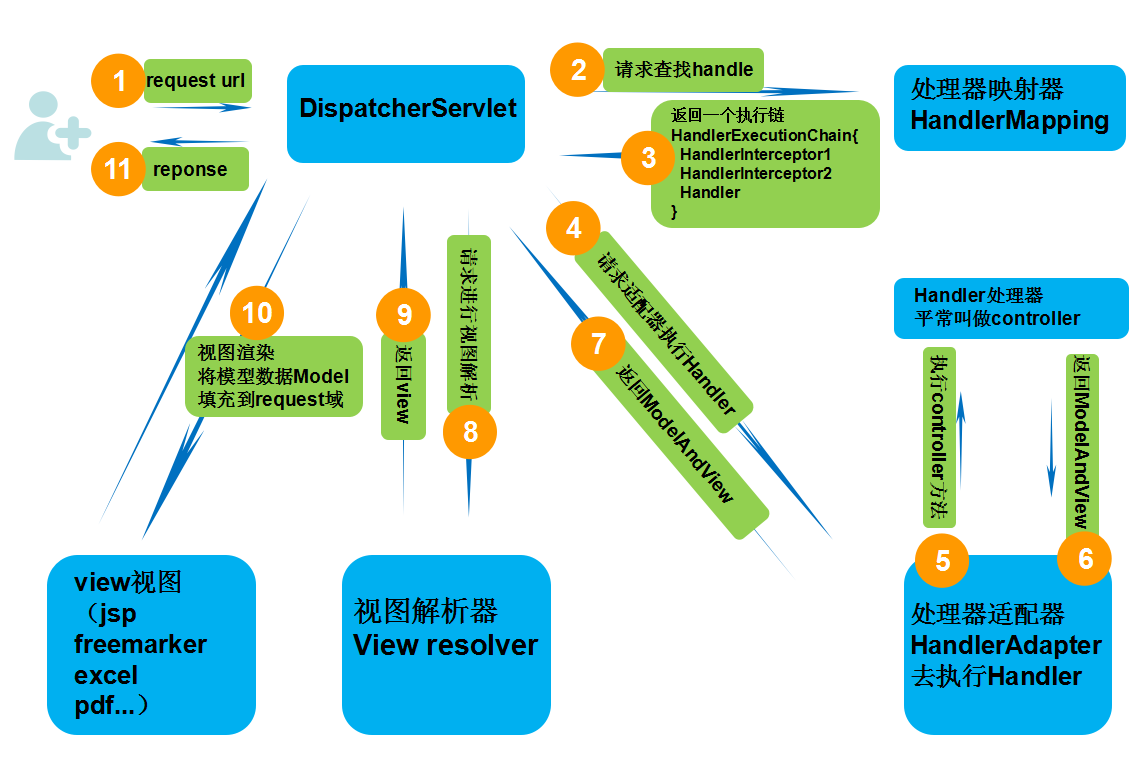
\includegraphics[width=0.7\linewidth]{figures/SpringModelAndView.png}
	\caption{}
	\label{fig:SpringModelAndView}
\end{figure}
	\subsubsection{第三个三级标题}
	
	
	\section{java基础}
	%\subsection{二级标题}
	\subsubsection{快速失败(fail-fast) 和 安全失败(fail-safe) 的区别是什么?}
	\begin{enumerate}
		\item java.util包下面的所有的集合类都是快速失败的, 而java.util.concurrent包下面的所有类都是安全失败的. 快速失败的迭代器会抛出ConcurrentModificationException异常, 而安全失败的迭代去永远不会抛出这样的异常.

	\end{enumerate}
\subsubsection{8种基本数据类型}
\begin{table}[!htbp]
	\centering
	\caption{实现}
	\begin{tabular}{|l|r|}
		
		\hline
		类型&大小(注释/包装类)\\
		\hline
		byte&8(Byte)\\
		\hline
		short&16(Short)\\
		\hline
		int&32(Integer)\\
		\hline
		long&64(Long)\\
		\hline
		float&32(Float)\\
		\hline
		double&64(Double)\\
		\hline
		char&16(Character)\\
		\hline
		boolean&8(Boolean)\\
		\hline
	\end{tabular}
\end{table}
\subsubsection{Comparable \& Comparator 区别}
Comparable 是接口 能力赋予
\begin{lstlisting}
public interface Comparable<T> {
	public int compareTo(T o);
}
\end{lstlisting}
Comparator 是外部比较器, 也是接口, 类似于 C++sort中自定义的cmp函数
\begin{lstlisting}
Collections.sort(list, new Comparator<Person2>() {
	public int compare(Person o1, Person o2) {
		return o1.getAge() - o2.getAge();
	}
})
\end{lstlisting}
\subsubsection{java采用值传递还是引用传递?}
采用值传递, 但是因为采用浅拷贝, 所以会修改传递的对象的相关属性.
\subsubsection{java深拷贝和浅拷贝}
实现了Coneable接口实现深拷贝.
\subsubsection{java"==" 和 equals 的区别}
1. "==" : 如果是基本数据类型, 则直接对值进行比较, 如果是引用数据类型, 则是对他们的地址进行比较;
\par
2. equals方法继承Object类, 在具体实现时可以覆盖父类中的实现. 看一下Object中equals的源码发现, 它的实现也是对\textbf{对象的地址}进行比较, 可以覆盖实现这个方法, 如果两个对象的类型一致, 并且内容一致, 则返回true.
\par
在实际开始中总结:
\par
(1) 类未复写equals, 则使用equals方法比较两个对象时, 相当于==比较, 及两个地址是否相等. 地址相等, 返回true, 地址不相等, 返回false.
\par
(2) 类复写equals方法, 走复写之后的判断方式. 通常, 我们会将equals复写成: 当两个对象内容相同时, 则equals返回true, 内容不同时, 返回false.
\par
对于set, hashMap, hashset等, 还要重写hashCode值, 比如set判断两个元素是否相等的时候, 会判断hashcode和equals都相等, 则认为相等, 不会添加新元素.
\subsubsection{String和StringBuilder, StringBuffer的区别}
String是不可变字符串对象(final的char数组), StringBuilder和StringBuffer(线程安全)是可变字符串对象.
\par
为什么String是final修饰的?
\par
1. 为了实现字符串池, 因为只有当字符串是不可变的, 字符串池才有可能实现.
\subsubsection{Java反射机制}
简单来说就是在, 运行状态中, 对于任意一个类, 都能够知道这个类的所有属性和方法; 对于任意一个对象, 都能够调用它的任意方法和属性; 并且能改变它的属性. 这种动态获取的信息以及动态调用对象的方法的功能称为Java语言的反射机制.
\par
优点: 代码灵活度提高
\par
缺点: 性能瓶颈, 性能较慢.
\subsubsection{简述面向对象三大特征, 继承, 封装, 多态}
1. 封装
\par
简单来说, 就是使用private方法将没有必要暴露的方法和属性进行隐藏.
\par
2. 继承
\par
继承是从已有的类中派生出行的类, 减少代码冗余. 
\par
3. 多态
\par
父类引用指向不同子类对象.
\subsubsection{红黑树}
一般考察红黑树: 只考察概念.
\begin{figure}
	\centering
	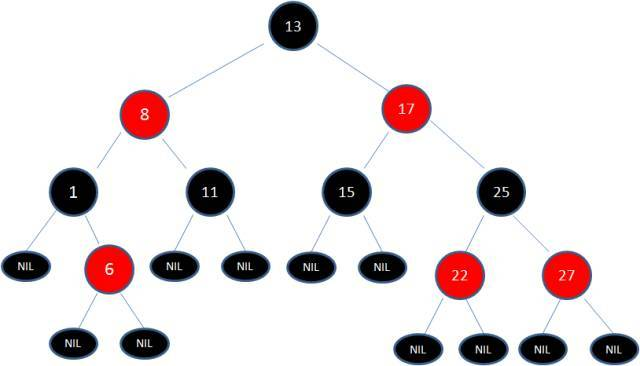
\includegraphics[width=0.7\linewidth]{figures/red_black.jpg}
	\caption{}
	\label{fig:jvm_copy}
\end{figure}
\begin{enumerate}
	\item 节点是红色或黑色
	\item 根节点是黑色
	\item 所有叶子都是黑色(叶子是NIL节点).
	\item 每个红色节点必须有两个黑色节点
	\item 从任一节点到其每个叶子的所有简单路径都包含相同数目的黑色节点.
	
\end{enumerate}

	\subsubsection{hashmap的数据结构}
	\begin{enumerate}
		\item jdk1.7 由 数组 + 链表  来构成
		\item jdk1.8 由 数组 + 链表 + 红黑树 来构成
		\item jdk1.8的时候, 当元素不超过64个的时候, 不会出现链表转红黑树, 当元素超过64个的时候, 会出现链表转红黑树.
		\item jdk1.8 当链表长度达到8个的时候, 链表会转为红黑树, 当红黑树元素长度退回到6个的时候会出现红黑树转为链表.
		\item jdk1.7 采用头插法, jdk1.8采用尾插法.
	\end{enumerate}
	\subsubsection{heap和stack有什么区别}
	\begin{enumerate}
		\item java的内存分为两类, 一类是堆内存, 一类是栈内存
		\item 栈内存是指程序进入一个方法时, 会为这个方法单独分配一块私属存储空间, 用于存储这个方法内部的局部变量. 当这个方法结束时, 分配给这个方法的栈会释放, 这个栈中的变量也随之释放.
		\item 使用new创建的对象存放在堆里, 不会随方法的结束二小时. 方法中的局部变量使用final修饰后, 放在堆中, 而不是栈中.
		
	\end{enumerate}

	\subsubsection{Array 和 ArrayList 的区别}
	\begin{enumerate}
		\item Array 大小固定, ArrayList 大小是动态变化的.
	\end{enumerate}
\subsubsection{Java各种锁: 悲观锁, 泪管所, 自旋锁, 偏向锁, 轻量/重量锁, 读写锁, 可重入锁}
悲观锁和乐观锁指的是并发情况下的两种不同策略, 是一种宏观的描述.
\par

\begin{enumerate}
	\item 悲观锁和乐观锁指的是并发情况下的两种不同策略, 是一种宏观的描述.
	
\end{enumerate}
\subsubsection{Collection 和 Collections 的区别}
\begin{enumerate}
	\item Collection 是集合类的上级接口, 继承他的接口主要是set和list
	\item Collections 类数针对集合类的一个帮助类. 它提供了一系列的静态方法对各种集合的搜索, 排序, 线程安全化等操作.
\end{enumerate}
\subsubsection{接口与抽象类区别}
\begin{enumerate}
	\item 类可以实现多个接口但只能继承一个抽象类
	\item 接口里面所有的方法都是Public的, 抽象类允许Private, Protected方法
	\item JDK接口可以实现默认方法和静态方法, 前面加defalut, static关键字.
\end{enumerate}
\begin{lstlisting}
public interface InterfaceJDK8 {
	
	/*接口的普通抽象方法*/
	public void common(String str);
	
	/*jdk1.8 默认方法:
	允许在已有的接口中添加新方法,而同时又保持了与旧版本代码的兼容性,
	默认方法与抽象方法不同之处在于抽象方法必须要求实现,但是默认方法则没有要求实现,
	相反,接口提供了一个默认实现,这样所有的接口实现者将会默认继承他
	(如果有必要的话,可以覆盖这个默认实现)。
	接口的默认方法:得到接口的实现类对象,直接用对象的引用.方法名。默认方法可以被实现类覆盖。
	*/
	default public void defaultMethod(String str){
		System.out.println("InterfaceJDK8:" + str);
	}
	
	/*jdk1.8 静态方法:
	允许在已有的接口中添加静态方法,接口的静态方法属于接口本身,不被继承,也需要提供方法的现。
	*/
	public static void staticMethod(String str){
		System.out.println("InterfaceJDK8:" + str);
	}
	
}
\end{lstlisting}
\subsubsection{ArrayList和LinkedList内部实现大致是怎样的? 他们之间的区别和优缺点}
\begin{enumerate}
	\item ArrayList: 内部使用数组的形式实现了存储, 利用数组的小表进行元素的访问, 因此对元素的随机访问速度非常快. 初始化大小为10, 插入新元素的时候, 会判断是否需要扩容, 扩容的步长是0.5倍原容量, 扩容方式是利用数组的复制, 因此有一定的开销
	\item LinkedList:内部使用双向链表的结构实现存储, LinkedList有一个内部类作为存放元素的单元, 里面有三个属性, 用来存放元素本身以及前后2个单元的引用, 另外LinkedList内部还有一个Header属性, 用来标识起始位置, LinkedList的第一个单元和最后一个单元都会指向header, 因此形成了一个双向链表结构.
\end{enumerate}
\subsubsection{==和equals的区别}
==是运算符, 而equals是Object的基本方法, ==用于基本数据的类型比较, 或者是比较两个对象的引用是否相同, equals用于比较两个对象的值是否相等, 例如字符串的比较.
\subsubsection{hashCode方法的作用}
\begin{enumerate}
	\item 如果两个对象equals方法相等, 那么hashCode一定相同
	\item 如果两个对象的hashCode相同, 并不表示两个对象相同(只能表示hash碰撞相同), equals方法相同.
\end{enumerate}
\subsubsection{反射}
简单来说, 在运行状态中, 对于任意一个类, 都能够知道这个类的所有属性和方法, 对于任意一个对象, 都能够调用他的任意方法和属性, 并且能够改变他的属性. 

\section{JVM}
%\subsection{二级标题}
\subsubsection{GC的三种收集方法: 标记清除, 标记整理, 复制算法的原理与特点, 分别用在什么地方, 如果让你优化收集方法, 有什么思路}
\begin{enumerate}
	\item 标记清除: 先标记, 标记完毕之后再清除, 缺点: 效率不高会产生碎片.
	\begin{figure}
		\centering
		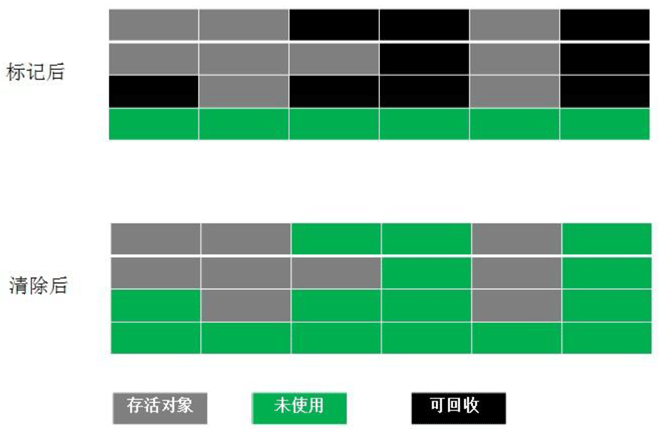
\includegraphics[width=0.7\linewidth]{figures/sign_remove.png}
		\caption{}
		\label{fig:sign_remove}
	\end{figure}
	\item 标记整理: 标记完毕之后, 让所有存活的对象向一端移动
	\item 复制算法: 分别8:1的Eden去和survivor区
	\begin{figure}
		\centering
		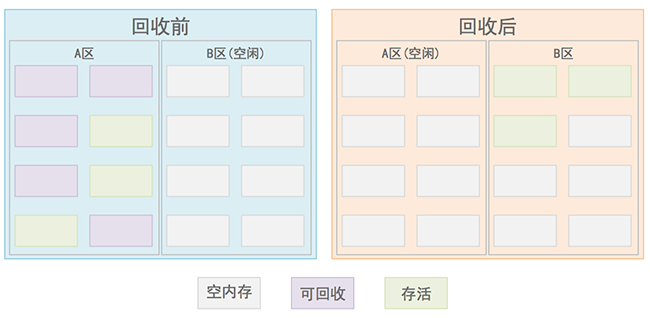
\includegraphics[width=0.7\linewidth]{figures/jvm_copy.jpg}
		\caption{}
		\label{fig:jvm_copy}
	\end{figure}
\end{enumerate}
\subsubsection{JVM的主要组成部分及其作用?}
JVM包含两个子系统和两个组件, 两个子系统为Class loader(类加载), Execution engin(执行引擎); 两个组件为 Runtime data area(运行时数据区), native Interface(本地接口)

\begin{enumerate}
	\item Class loader: 根据给定的额全限定类名(如:java.lang.object)来装在class文件到Runtime data area中的method area.
	\item Execution engine(执行引擎): 执行classes中的指令
	\item native Interface(本地接口): 与native libraries交互, 是其他编程语言交互的接口.
	\item Runtime data area(运行时数据区): 这就是我们常说的jvm的内存
\end{enumerate}
\par
\textbf{作用:} 首先通过编译器吧java代码转换成字节码, 类加载器(ClassLoader) 再把字节码加载到内存中, 将其放在运行时数据区(Runtime data area)的方发区内, 而字节码文件知识jvm的一套指令集规范, 并不能直接交给底层操作系统去执行, 因此需要特定的命令解析器执行引擎(Execution Engine), 将字节码翻译成底层系统指令, 在交由CPU去执行, 而这个过程中需要调用其他语言的本地库接口(Native Interface) 来实现整个程序的功能. 
\par
Java程序运行机制步骤
\begin{enumerate}
	\item 编码: IDEA等IDE进行编码java, 后缀.java
	\item 编译: javac 将源代码编译成字节码文件,字节码文件的后缀名为.class
\end{enumerate}
类的加载是将类的.class文件中的二进制数据读入到内存中, 将其放在运行时数据区的方法去内, 然后在堆区创建一个java.lang.Class对象, 用来封装类在方区内的数据结构.
\subsubsection{JVM运行时数据区}
运行时数据区由如下几个区域构成
\begin{enumerate}
	\item 程序计数器(PC): 当前线程所执行字节码的行号指示器, 字节码解析器的工作是通过改变这个计数器的值, 来选去下一条需要执行的字节码指令.
	\item java虚拟机栈(Java Virtual Machine Stacks): 用于存储局部变量表, 操作数栈, 动态链接, 方法出口等信息.
	\item 本地方法栈(Native Method Stack) : 与虚拟机栈的作用是一样的, 只不过虚拟机栈是服务Java方法的, 而本地方法栈是为虚拟机调用Native方法服务的.
	\item Java堆(Java Heap): Java 虚拟机中内存最大的一块, 是被所有线程共享的, 几乎所有的对象实例, 都在这里分配内存;
	\item 方法区(Method Area): 用于存储已被虚拟机加载的类信息, 常量, 静态变量, 及时编译后的代码等数据.
\end{enumerate}
\subsubsection{永久代PermGen 和 元空间Metaspace 区别}
\begin{enumerate}
	\item 永久代PermGen : 是jdk1.7 对于方发区的实现. 由于动态生成类的情况比较容易出现永久代的内存溢出, 抛出异常.
	\item 元空间MetaSpace: 存在于本地内存.
\end{enumerate}
\subsubsection{说一下堆栈的区别?}
\textbf{物理地址}
\par
堆的物理地址分配对对象是不连续的. 因此, 性能慢些. 在GC的时候也要考虑到不连续的分配, 所以后各种算法. 比如, 标记-清除, 复制, 标记压缩, 分代(即新生代生活复制算法, 老年代使用标记压缩算法);
\par
栈使用的是数据结构中的栈, 先进后出的原则, 物理地址分配是连续的. 所以性能快.
\par
\textbf{内存区别}
\par
堆因为是不连续的, 所以分配的内存是在\textbf{运行期}确认的, 因此大小不固定. 一般堆大小远大于栈.
\par
栈是连续的, 所以分配的内存大小要在编译器就确认, 大小是固定的.
\par
\textbf{程序的可见度}
\par
堆对于整个应用程序都是共享, 可见的.
栈只对于线程是可见的. 所以也是线程私有. 他的生命周期和线程相同.
TIPS:
\begin{enumerate}
	\item 静态变量放在方法区.
	\item 静态的对象还是放在堆.
\end{enumerate}

\subsubsection{对象的访问定位?}
目前主流的访问方式有句柄和直接指针两种方式.

\begin{enumerate}
	\item 指针: 指向对象, 代表一个对象再内存中的起始地址
	\item 句柄: 可以理解为指向指针的指针, 维护者对象的地址. 句柄不直接指向对象, 而是指向对象的地址(句柄不发生变化, 指向固定内存你地址), 再由对象的指针指向对象的真实内存地址.
\end{enumerate}
\textbf{句柄访问}
\par
Java堆中划分出一块内存作为句柄池, 引用中存储对象的句柄地址, 而句柄中包含了\textbf{对象实例数据}与\textbf{对象类型数据}各自的决堤地址信息, 具体构造如下图所示:
\begin{figure}
	\centering
	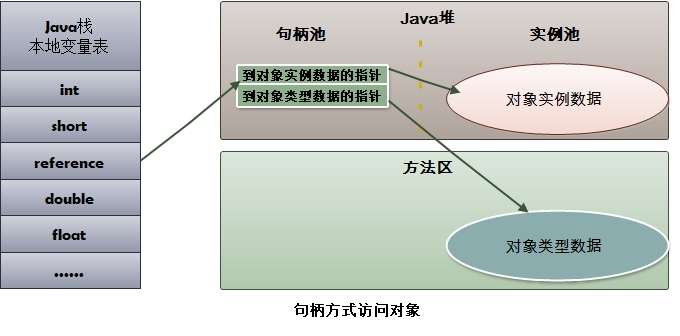
\includegraphics[width=0.7\linewidth]{figures/jvm_handler.jpg}
	\caption{}
	\label{fig:jvm_handler}
\end{figure}
\textbf{直接指针}
\par
\begin{figure}
	\centering
	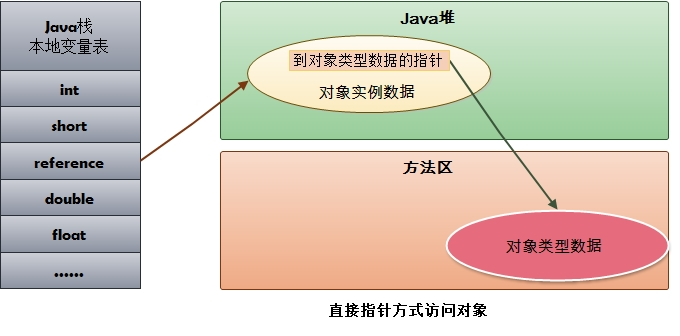
\includegraphics[width=0.7\linewidth]{figures/jvm_point.jpg}
	\caption{}
	\label{fig:jvm_point}
\end{figure}
\subsubsection{垃圾回收器的基本原理是什么?}
\textbf{可达性分析}
\par
GC采用有向图的方式记录和管理堆中的所有对象. 通过这种方式确定哪些对象是"可达的", 哪些对象是"不可达的", 当GC确定一些对象为"不可达"时, GC就有责任回收这些内存空间.
程序员可以手动执行System.gc(), 通知GC运行, 但是Java语言规范并不保证GC一定会执行.
\par
\textbf{引用计数法}
为每个对象创建一个引用技术, 有对象引用时计数器+1, 引用被释放是技术-1, 当计数器为0时就可以被回收. 优缺点, 不能解决循环引用的问题.
\subsubsection{在java中, 对象什么时候可以被垃圾回收?}
当对象边的不可触及的时候, 这个对象就可以被回收了, 垃圾回收不会发生在永久代, 如果永久代满了或者是超过了临界值, 会触发完全垃圾回收(full gc), 会导致Stop-the-world. 
\section{Redis}
%\subsection{二级标题}
\subsubsection{什么是Redis?}
\begin{enumerate}
	\item 高性能非关系型数据库
	\item 可以存储五种不同类型的额值之间的映射. 键的类型只能为字符串, 值支持五种类型数据:字符串(string), 列表(list), 集合(set), 散列表(hash), 有序集合(sorted set).
	\item redis数据是存在内存中的, 所以读写速度非常快.
\end{enumerate}
\subsubsection{简述Redis单线程模型?}
实现方式
\par
(1) I/O多路复用
\par
简单来说, 可以使用I/O多路复用来坚定多个socket连接, 然后将感兴趣的时间注册到内核中并监听每个事件是否发生. 
\par
(2) 基于事件驱动
\par
服务器需要处理两类事件, 文件事件; 时间事件.
\par
当被监听的套接字准备好执行连接应答(accept), 读取(read), 写入(write), 关闭(close)等操作时, 与操作相对应的文件事件就会产生, 这时文件事件处理器就会调用套接字之前关联好的事件处理器来处理这些事件.
\par
文件事件处理器(file event handler) 主要包含4个部分: 多个socket(客户端链接), IO多路复用, 文件事件分派; 事件处理;
\begin{figure}
	\centering
	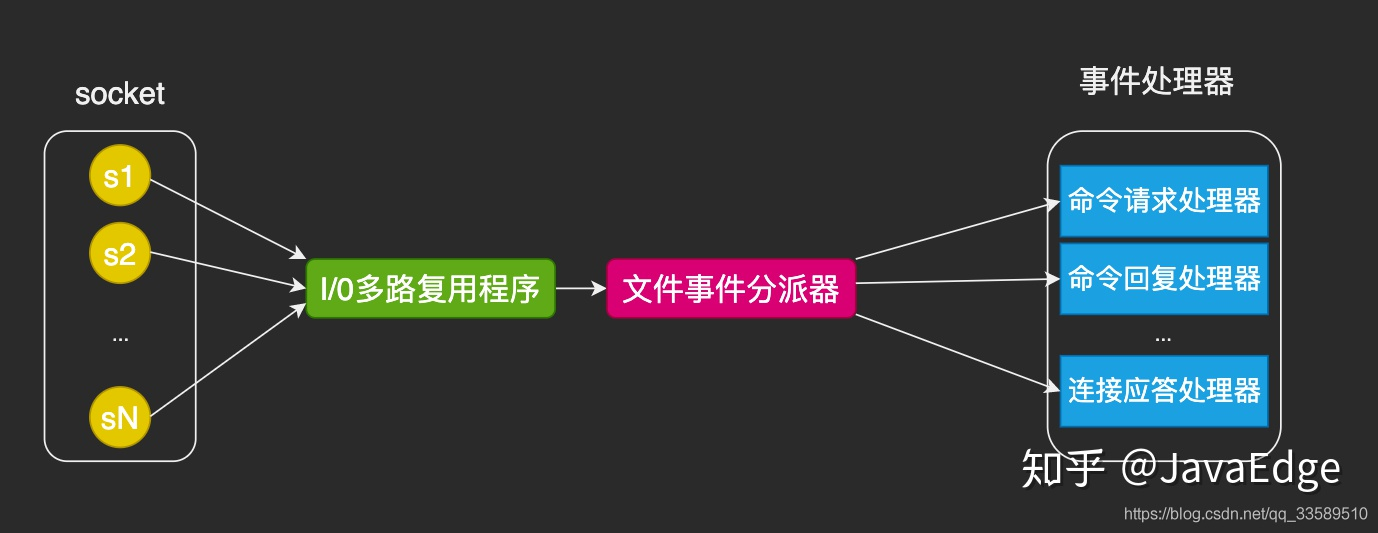
\includegraphics[width=0.7\linewidth]{figures/redis_file_event.jpg}
	\caption{}
	\label{fig:redis_file_event}
\end{figure}
\subsubsection{Redis五种类型数据的实现方式}
\begin{table}[!htbp]
	\centering
	\caption{实现}
	\begin{tabular}{|l|r|}
		
		\hline
		类型&编码\\
		\hline
		STRING&INT(整形, 在String中存储整形会是的)\\
		\hline
		STRING&EMBSTR(简单动态字符串, 对于短小的string(44位字符)会使用这种结构)\\
		\hline
		STRING&RAW(简单动态字符串, 对于稍微长一点的string会使用(44位字符)这种结构)\\
		\hline
		LIST&QUICKLIST(快表)\\
		\hline
		LIST&LINKEDLIST(快表)\\
		\hline
		SET&INTSET(整数集合)\\
		\hline
		SET&HT(哈希表)\\
		\hline
		ZSET&ZIPLIST(压缩列表)\\
		\hline
		ZSET&SKIPLIST(跳表)\\
		\hline
		HASH&ZIPLIST(压缩列表)\\
		\hline
		HASH&HT(哈希表)\\
		\hline
	\end{tabular}
\end{table}
字符串结构SDS和C中char[]有什么不同
\begin{enumerate}
	\item 获取SDS中字符串的长度因为SDS中存储了字符串的长度len属性, 直接访问, 时间复杂度O(1), 对于C语言获取字符串的长度需要经过遍历, 时间复杂度O(n).
	\item 避免缓冲区溢出, 会检查SDS中属性, free(空闲空间)能够实现字符串的扩充判断. 不足会重新申请空间.
	\item SDS支持空间预分配, 扩展的内存比实际需要的多
	\item SDS支持空间惰性释放, 字符串缩短之后, 不立即进行空间回收操作. SDS也提供相应API, 可以对冗余空间进行回收.
	\item 可以存储二进制, 因为SDS不以回车符号进行终止的判定.
\end{enumerate}
\subsubsection{redis字典的底层实现hashTable相关问题}
\begin{enumerate}
	\item 解决冲突: 链地址法, 即使用数组+链表的方式实现. 
	\item 扩容: 有两个指针h[0] 和 h[1], h[1] 用来备份, 当h[0], 满了使用渐进值hash, 插入都插入h[1], 查找两个表都进行查找.
\end{enumerate}
\subsubsection{压缩链表原理ziplist}
连续内存, 包含多个节点entry.
\begin{figure}
	\centering
	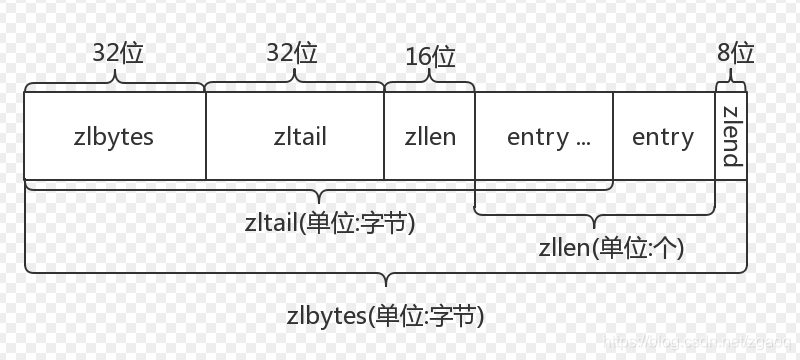
\includegraphics[width=0.7\linewidth]{figures/ziplist.png}
	\caption{}
	\label{fig:ziplist}
\end{figure}
\subsubsection{zset}
本质是舵机链表并有序.
skiplist与平衡树, 哈希表的比较
\begin{enumerate}
	\item skiplist和各种平衡树的元素排序是有序 的, 而哈希表不是有序的, 因此, 在哈希表上智能做单个key的查找, 不适宜做范围查找.
	\item 在做范围查找的时候, 平衡树比skiplist操作要复杂. 在平衡树上, 需要做一步回退操作. 而在skiplist上进行范围查找就非常简单, 只要找到最小值之后对第一层链表进行若干部遍历就可以实现.
	\item 平衡树插入和删除操作, 会引起结构调整, 操作复杂, skiplist的插入和删除只需要修改相邻节点的指针, 操作简单又快速.
\end{enumerate}

\subsubsection{AOF和RDB两种持久化方式区别}
\begin{enumerate}
	\item AOF存储命令, RDB存储数据.
	\item AOF文件因为存储命令, 所以在redis启动的时候加载aof会比加载rdb要慢. 
	\item Redis 4.0 之后 启动了混合模式, AOF不需要是全量日志, 只要保存前一次RDB存储开始到这段时间增量AOF日志即可.
\end{enumerate}
\subsubsection{Redis中过期策略和缓存淘汰机制}
\begin{enumerate}
	\item 定期删除: redis默认每隔100ms随机对key检查, 有过期的key则进行删除. 容易导致很多过期的key没被发现
	\item 惰性删除: 获取某个key的时候, redis会检查一下, 如果过期了就进行删除.
\end{enumerate}
\subsubsection{为什么要使用Redis}
\begin{enumerate}
	\item 高性能: 内存的读取比硬盘乃至固态硬盘的读取速度都要快得多
	\item 高并发: 直接操作缓存能够承受的请求是远远大于直接访问数据库的, 所以我们可以考虑把数据库中的部分数据转移到缓存中去, 这样用户的一部分请求会直接请求缓存这里而不用经过数据库. 
	\item 高性能: 使用多路I/O复用木星, 非阻塞IO;
\end{enumerate}
\subsubsection{Redis底层实现跳表介绍一下}
跳表是带多级索引的链表, 时间复杂度O(lgn), 所能实现的功能和红黑树差不多, 但是跳表有一个区间查找的优势, 红黑树没有.
\begin{figure}
	\centering
	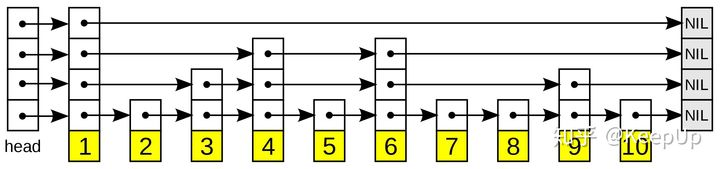
\includegraphics[width=0.7\linewidth]{figures/jump_table.jpg}
	\caption{}
	\label{fig:redissharding}
\end{figure}
\begin{enumerate}
	\item 表头: 负责维护跳表的节点指针.
	\item 跳跃表节点: 保存着元素值, 以及多个层.
	\item 层: 保存着指向其他元素的指针, 高层的指针越过的元素数量大于等于底层的指针, 为了提高查找效率, 程序总是从高层先开始访问, 然后随着元素值范围的缩小, 慢慢降低层次.
	\item 表尾: 全部由NULL组成.
\end{enumerate}

\subsubsection{为什么要使用Redis而不用map/guavaCache做缓存}
\begin{enumerate}
	\item guavaCache实现的是本地缓存, 最主要的特点是轻量化以及快速, 生命周期随着jvm的销毁而结束, 冰洁在多实例的情况下, 每个实例都需要个字保存一份缓存, 缓存容易出现不一致性.
	\item 使用redis之类的缓存称为分布式缓存, 在多实例的情况下, 各实例公用一份缓存数据, 缓存具有一致性.
\end{enumerate}
\subsubsection{分布式锁如何使用redis实现}
\begin{enumerate}
	\item setnx命令原子性实现. 
\end{enumerate}
\subsubsection{Redis的内存淘汰策略有哪些}
Redis的内存淘汰策略是指在Redis用于缓存的内存不足时, 怎么处理需要新写入且需要申额外空间的数据.
全局的键空间选择性移除
\begin{enumerate}
	
	\item noeviction: 当内存不足以容纳新写入数据时, 新写入操作会报错.
	\item allkeys-lru: 当内存不足以容纳新写入数据时, 在键空间中, 移除最近最少使用的key.
	\item allkeys-random: 当内存不足以容纳新写入数据时, 在键空间随机移除某个key.
\end{enumerate}
设置过期时间的键空间选择性移除
\begin{enumerate}
	
	\item volatile-lru: 当内存不足以容纳新写入数据时, 在设置了过期时间的键空间中, 移除最近最少使用的key.
	\item volatile-random: 当内存不足以容纳新写入数据时, 在设置了过期时间的键空间中, 随机移除某个key.
	\item volatile-ttl: 当内存不足以容纳新写入的数据时, 在设置了过期时间的键空间中, 有更早过期时间的key优先移除. 
\end{enumerate}
\subsubsection{Redis事物的概念}
Redis事物的本质通过MULTI, EXEC, WATCH等一组命令的集合. 
\begin{enumerate}

	\item 事物开始 MULTI
	\item 命令入队
	\item 事务执行 EXEC
\end{enumerate}
* 事务执行过程中, 如果服务端收到有EXEC, DISCARD, WATCH, MULTI之外的请求, 将会把请求放入队列中排队.
简单介绍一下watch, 当watch的变量在事务过程中发生了改变, 那么事务失败, 拒绝执行事物.
\begin{lstlisting}
	>watch 'name'
	>multi
	>set "name" "peter"
	>exec
	(nil)
\end{lstlisting}
\subsubsection{RedisSharding}
简单来说就是多个client 连接多个redis, 然后通过一致性哈希算法, 来确定访问的key+访问的客户端名字在哪一台redis上.
采用的算法是MURMUR\_HASH, 
\begin{figure}
	\centering
	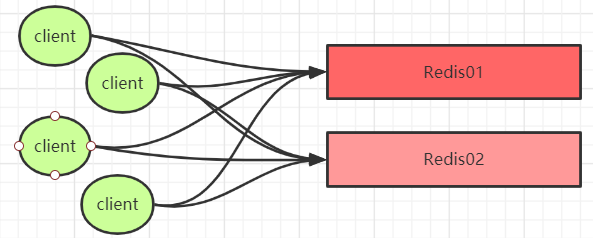
\includegraphics[width=0.7\linewidth]{figures/redis_sharding.png}
	\caption{}
	\label{fig:redissharding}
\end{figure}
\subsubsection{缓存雪崩}
缓存同一时间大面积的失效, 所以, 后面的请求都会落到数据库上, 造成数据库短时间内承受大量请求而崩掉

\par
\textbf{解决方案}
\begin{enumerate}
	
	\item 缓存数据的过期时间设置随机, 防止同一时间大量数据过期现象发生.

\end{enumerate}

\subsubsection{缓存穿透}
缓存和数据库中都没有数据, 导致所有的请求都落在数据库中, 造成数据库短时间内承受大量请求而崩掉.
\par
\textbf{解决方案}
\begin{enumerate}
	
	\item 从缓存中取不到的数据, 在数据库中也没有取到, 这时也可以将key-value对写为key-null, 缓存时间设定为30s.
	
\end{enumerate}

\subsubsection{缓存击穿}
缓存中没有但数据库中有的数据, 由于并发用户特别多, 同时读缓存没读到数据, 又同时去数据库取数据, 引起数据库压力瞬间增大, 造成过大压力, 和缓存雪崩不同的是, 缓存击穿指并发查询同一条数据, 缓存雪崩是不同数据都过期了, 很多数据都查不到, 从而查数据库.
\par
\textbf{解决方案}
\begin{enumerate}
	\item 设置热点数据永不过期	
\end{enumerate}
\subsubsection{缓存预热}
系统上线后, 将相关的缓存数据直接加载到缓存系统. 这样就可以避免在用户请求的时候, 先查询数据库, 然后再讲数据缓存的问题, 用户直接查询事先被预热的缓存数据.
\par
\textbf{解决方案}
\begin{enumerate}
	\item 定时刷新缓存;	
\end{enumerate}
\subsubsection{Redis6.0 为什么要引入多线程呢?}
Redis将所有数据放在内存中, 内存的相应市场大约100ns, 对于小数据包, Redis服务器可以处理8w到10wQPS, 这也是Redis处理的极限了, 对于80\%的公司来说, 单线程的redis已经足够使用了. 
\par
但随着越来越复杂的业务场景, 需要更大的QPS.
\begin{enumerate}
	\item 可以充分利用服务器CPU资源, 目前主线程只能利用一个核
	\item 多线程任务可以分摊Redis同步IO读写负荷.	
\end{enumerate}
\subsubsection{Redis主从复制模式}
\begin{enumerate}
	\item 完全同步:刚开始, 主服务器发送RDB文件给从服务器, 实现主从同步.
	\item 部分同步:当连接由于网络原因断开的时候, 将中间断开的执行的写命令发送给从服务器. 实现同步.	
\end{enumerate}
\subsubsection{Redis中持久化机制}
\begin{enumerate}
	\item 
\end{enumerate}


\section{计算机网络}
%\subsection{二级标题}
\subsubsection{计算机网络分层}
计算机网络OSI模型是七层, 如果是TCP/IP
应用层(HTTP/FTP) - 应用层
\par 
~ - 表示层
~ - 会话层
\par
传输层(UDP/TCP) - 传输层
\par
网际层(IP) - 网络层
\par 
主机至网络层 - 数据链路层
~ - 物理层
\subsubsection{TCP和UDP区别?}
\par
UDP: 面向报文, 支持1对1, 1对多, 多对1的交互通信
\par
TCP: 面向连接, 提供可靠交付, 有流量控制, 拥塞控制, 提供全双工通信, 面向字节流. TCP是点对点的.
\subsubsection{TCP三次握手相关问题}
为什么三次握手而不是两次握手: 主要是为了防止已失效的链接请求报文段突然又传送到了B, 因而产生错误. 如果只要两次握手就建立连接, 那么如果A第一次请求丢失了, A 又发送了一次请求, 但是这一次传输结束了, A上一次丢失的请求再次被传送到了B, 如果建立了连接, 但是A现在一直不回应B, 导致B浪费了资源.
\subsubsection{TCP四次挥手问题}
关闭连接的时候, 当Server端收到FIN报文时候, 很可能并不会立即关闭SOCKET, 所以只能先回复一个ACK报文, 告诉Client端, 你发送的FIN我收到了, 只有等我Server端所有的报文都发送完了, 我才能发送FIN报文. 不能一起发送, 所以需要四步挥手.
\subsubsection{TCP协议-如何保证传输的可靠性}
\textbf{超时重传:} 简单理解就是发送在发送完数据后等待一个时间, 时间到大没有接收到ACK报文, 那么对刚才发送的数据进行重新发送
\par
\textbf{连接管理:} 使用三次握手和四次挥手
\par
\textbf{流量控制:} TCP根据接收端对数据的处理能力, 决定发送端的发送速度, 这个机制就是流量控制. TCP协议的包头信息当中, 有一个16位字段的窗口大小, 发送方更具ACK报文里的窗口大小的值的改变自己的发送数据
\par
\textbf{拥塞控制:} 慢开始, 拥塞避免, 快重传, 快恢复.
\par
慢开始算法的思路就是, 不要一开始就发送大量的数据, 先探测一下网络的拥塞程度, 也就是说由小到大主键增加拥塞窗口的大小.
\par
拥塞避免算法让拥塞窗口缓慢增长, 即每经过一个往返时间RTT就把发送方的拥塞窗口cwnd加1, 而不是加倍. 这样拥塞窗口按线性归路缓慢增长.
\par
快重传和快恢复: 发送方只要一脸收到三个重复确认就引动立即重传对方尚未收到的报文段, 而不必继续等待设置的重传计时器时间到器.
\begin{figure}
	\centering
	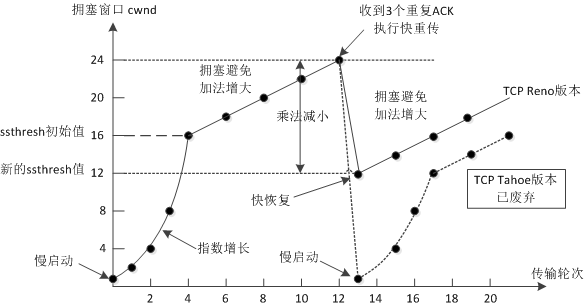
\includegraphics[width=0.7\linewidth]{figures/tcp.png}
	\caption{}
	\label{fig:tcp}
\end{figure}
\subsubsection{Cookie作用, 安全性问题和Session的比较}
(1) Cookie是服务器发送到用户浏览器并保存在本地的一小块数据,  他会在浏览器之后向统一服务器再次发送请求时被携带上.
\par
(2) Session 存储在服务器端. 使用Session维护用户登录状态的过程如下: (需要cookie作为传输机制)
用户进行登陆是, 用户提交包含用户名和密码的表单, 放入HTTP请求报文中;
服务器校验该用户名和密码, 如果正确则把用户信息存储到Redis中, 他在Redis中的key成为SessionId.
\par
服务器返回的响应报文Set-Cookie首部字段包含了这个SessionID, 客户端收到响应报文之后将该Cookie值存入浏览器中.客户端之后对同一个服务器进行请求时会包含该Cookie值, 服务器收到之后提取出SessionID, 从Redis中取出用户信息, 继续之前的业务操作.
\par
session 的运行依赖 session id, 而 session id 是存在 cookie 中的, 也就是,如果浏览器禁用了 cookie, 同时 session 也会失效(但是可以通过其它方式实现, 比如在 url 中传递 session\_id)
\par
cookie存在大小限制, 单个不超过4k, 浏览器中Cookie个数也有限制.
Session没有大小限制, 是和服务器内存有关的.
\subsubsection{}
\section{mysql}
%\subsection{二级标题}
\subsubsection{隔离级别}
\par
读已提交(read committed): 简单来说select * from account, 读出来的数据都是已经提交的数据.
\par 可以出现不可重复读(一个事物两次读到的事物不一样)和幻读(插入一条记录)
\par 
读未提交(read uncommitted) : 简单来说 select * from account, 读出来的数据是另一个事物还没有提交的数据, 
\par 可以出现脏读(无论是脏写还是脏读,都是因为一个事务去更新或者查询了另外一个还没提交的事务更新过的数据。因为另外一个事务还没提交,所以它随时可能会回滚,那么必然导致你更新的数据就没了,或者你之前查询到的数据就没了,这就是脏写和脏读两种场景。): 简单的说, 就是A事物在还没commit数据的情况下, b事物使用了A事物的数据, 但是A事物出现了回滚操作, 导致B事物读出来的数据是脏数据. 可以出现不可重复度, 可以出现幻读. (感觉是最不靠谱的一个级别)
\par 
可重复读(RR: Repeatable read) : 简单来说, 就是A事物插入了一条新数据, B事物没看到, 因为可重复读, 但是B是可以操作这条新数据的. 
\par 
串行化(serializable): 只能一个一个处理, 没什么问题, 但是效率太低一般不考虑.
\par 提示: 不可重复读对应的是修改即Update,幻读对应的是插入即Insert.
\par TIPS:
可见,幻读就是没有读到的记录,以为不存在,但其实是可以更新成功的,并且,更新成功后,再次读取,就出现了。
\subsubsection{ACID}
原子性: 不可分割
\par
一致性: 数据完整性, 例如金钱的综述
\par
隔离性: 不被打扰
\par
持久性: 永久保存




	\section{附录: 相关样例}
	第一个公式
	\begin{equation}
		F=ma=aa
	\end{equation}
	我们可以知道牛顿得出了与物体质量和加速度之间的关系$F=ma$
	换行公式:
	\begin{align}
		y &=ax\notag\\
		&=bx
	\end{align}
	
	\subsubsection{小练习}
	\begin{equation}
		v=\frac{x}{y}
	\end{equation}
	\begin{equation}
		y=e^{x}
	\end{equation}
	\begin{equation}
		y=ax^2+bx+c
	\end{equation}
	\begin{equation}
		F=G\frac{Mm}{r^2}
	\end{equation}
	\begin{equation}
		y=4\pi \frac{\sin{x}}{\ln{x^2}}
	\end{equation}
	\begin{equation}
		y=\sum^{n}_{i=1} x^2+1
	\end{equation}
	\begin{equation}
		i=\int_{1}^{2}x^2+\tan{x}\mathrm{d}x
	\end{equation}
	
	\begin{equation}
		A=\begin{bmatrix}
			1&1&3\\4&5&6\\5&6&7&\\
		\end{bmatrix}
	\end{equation}
	\subsubsection{三级标题}
	
	接下来将开始书写正文
	\begin{enumerate}
		\item 第一个问题:
		\item 第二个问题:
		\item 第三个问题:
	\end{enumerate}
	
	\subsubsection{第二个三级标题}
	
	
	\subsubsection{第三个三级标题}
	
	\section{公式的写作}
	第一个公式
	\begin{equation}
		F=ma
	\end{equation}
	我们可以知道牛顿得出了与物体质量和加速度之间的关系$F=ma$
	
	换行公式:
	\begin{align}
		y &=ax\notag\\
		&=bx
	\end{align}
	
	\subsubsection{练习}
	\begin{equation}
		v=\frac{x}{y}
	\end{equation}
	\begin{equation}
		y=e^{x}
	\end{equation}
	\begin{equation}
		y=ax^2+bx+c
	\end{equation}
	\begin{equation}
		F=G\frac{Mm}{r^2}
	\end{equation}
	\begin{equation}
		y=4\pi \frac{\sin{x}}{\ln{x^2}}
	\end{equation}
	\begin{equation}
		\label{eq:ceshi}
		y=\sum^{n}_{i=1} x^2+1
	\end{equation}
	
	现在引用(\ref{eq:ceshi})
	
	\begin{equation}
		i=\int_{1}^{2}x^2+\tan{x}\mathrm{d}x
	\end{equation}
	
	\begin{equation}
		A=\begin{bmatrix}
			1&1&3\\4&5&6\\5&6&7&\\
		\end{bmatrix}
	\end{equation}
	
	\begin{equation}
		A=\begin{cases}
			&x^2\\&x^2+x\\
		\end{cases}
	\end{equation}
	
	\subsubsection{表格的插入}
	
	\begin{table}[!htbp]
		\centering
		\caption{标题}
		\begin{tabular}{|l|c|r|}
			
			\hline
			指标1&指标2&指标3\\
			\hline
			居左&居中&居右\\
			\hline
		\end{tabular}
	\end{table}
	
	
	\begin{table}[!htbp]
		\centering
		\caption{标题}
		\begin{tabular}{ccc}
			\toprule
			数据&1&2\\
			\midrule
			甲方&600&700\\
			乙方&800&900\\
			\bottomrule
		\end{tabular}
	\end{table}
\end{document}
